\documentclass[a4paper]{article}

%------------------------------------------------------------
\usepackage[a4paper, total={6in, 9in}]{geometry}
\usepackage{amsmath, amssymb}
\usepackage{booktabs}
\usepackage{caption}
\usepackage{enumitem}
\usepackage{graphicx}
\usepackage{float}
\usepackage{inconsolata}
\usepackage{listings}
\usepackage{mathtools}
\usepackage{pstricks-add}
\usepackage{siunitx}
\usepackage[most]{tcolorbox}
\usepackage{tikz, pgfplots}
\usepackage{epstopdf} %converting to PDF
\usepackage{hyperref}
\usepackage{xfrac}

\usetikzlibrary{shapes.geometric}
\usetikzlibrary{arrows}
\usetikzlibrary{calc}

%------------------------------------------------------------
\graphicspath{{./fig/}}
\pgfplotsset{compat=1.13}
%------------------------------------------------------------
\setlength{\parindent}{0in}

\lstdefinestyle{C++}{
	language=C++,
	basicstyle=\ttfamily,
	keywordstyle=\color{blue}\ttfamily,
	stringstyle=\color{red}\ttfamily,
	commentstyle=\color{green}\ttfamily,
	morecomment=[l][\color{magenta}]{\#},
	showstringspaces=false
}

%------------------------------------------------------------
\newtcblisting[auto counter]{sexylisting}[2][]{sharp corners, 
    fonttitle=\bfseries, colframe=gray, listing only, 
    listing options={basicstyle=\ttfamily,language=C++}, 
    title=Listing \thetcbcounter: #2, #1}

%------------------------------------------------------------
\lstset{language=C++,
        basicstyle=\ttfamily,
        keywordstyle=\color{blue}\ttfamily,
        stringstyle=\color{red}\ttfamily,
        commentstyle=\color{green}\ttfamily,
        morecomment=[l][\color{magenta}]{\#},
        showstringspaces=false
}
%------------------------------------------------------------
\tikzstyle{block} = [draw, fill=blue!20, rectangle, 
    minimum height=3em, minimum width=3em]
\tikzstyle{sum} = [draw, fill=blue!20, circle, node distance=1cm]
\tikzstyle{input} = [coordinate]
\tikzstyle{output} = [coordinate]
\tikzstyle{pinstyle} = [pin edge={to-,thin,black}]

%------------------------------------------------------------
\newlength{\arrow}
\settowidth{\arrow}{\scriptsize$1000$}

\newcommand*{\myrightarrow}[1]{\xrightarrow{\mathmakebox[\arrow]{#1}}}

\newcommand{\uvec}[1]{\boldsymbol{\hat{\textbf{#1}}}}

%------------------------------------------------------------

\begin{document}
\title{ENG252 Dynamics: Practical 3}
\author{Shane Reynolds}
\maketitle

\section{Introduction}
\subsection{Moment of Inertia}
Consider a body with mass $m$ undergoing rotational motion, with angular acceleration $\alpha$, around a fixed axis $OO'$. Graphically this scenario is depicted in Figure 1. If we want to calculate the Moment of this body around the axis $OO'$, then we need to consider the moments of each and every infinitesimally small mass particle that make up the body. The moment of a single particle mass is given by:
\begin{equation}
M = \boldsymbol{r} \times \boldsymbol{F}
\end{equation}

We note $\boldsymbol{r}$ is the position vector of the particle from point where the moment is to calculated, and $\boldsymbol{F}$ is the force acting on the particle. If our motion is constrained to a 2D plane, equation (1) simplifies to the well known equation:
\begin{equation}
M = F \times d
\end{equation}
The quantity $F$ is the scalar magnitude of the force acting orthogonal to the shortest line connecting the particle mass to the moment point of calculation; and $d$ is the distance between between these two points. Using (2) we can calculate the moment $M_O$ about axis $OO'$ for a small mass element, $dm$, of the body in Figure 1:
\begin{equation}
	M_O = Fr = a_t \ dm \ r 
\end{equation}

\begin{figure}[h]
	\centering
	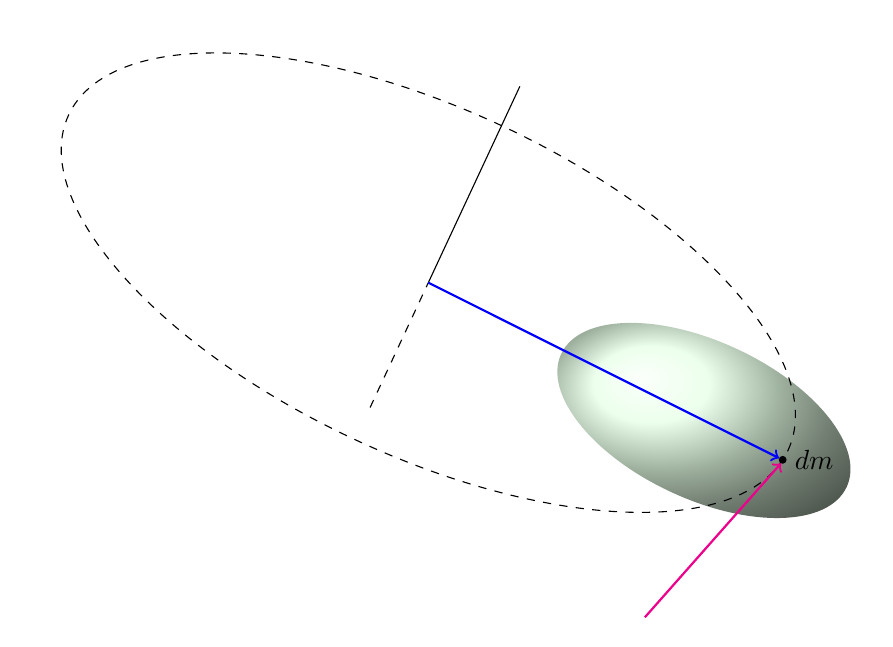
\begin{tikzpicture}
		\shade[ball color=green!10!, rotate=-25] (0,0) coordinate(C) ellipse (2 and 1);
		\fill[color=black] (1,-0.5) circle (0.05); 
		\draw[rotate around={-25:(-3.5,1.75)}] (-3.5,1.75) -- (-3.5,4.5);
		\draw[dashed, rotate around={-25:(-3.5,1.75)}] (-3.5,0) -- (-3.5,1.75);
		\draw[->, color=blue, thick] (-3.5,1.75) -- (0.9546,-0.4788);
		\draw [dashed, rotate around={-25:(-3.5,1.75)}] (-3.5,1.75) ellipse (5.04 and 2.2);
		\draw [->, color=magenta, thick] (-0.75,-2.5) -- (0.9788,-0.545);
		\node at (1.4,-0.5) {$dm$};
	\end{tikzpicture}
	\caption{A body of mass $m$ rotating about a fixed axis $OO'$ with some angular acceleration $\alpha$.}
\end{figure}

According to Giancoli a particle undergoing fixed axis rotation can re-express tangential acceleration $a_t$, as $\alpha r$, where $r$ is the distance from the centre of rotation to the particle. We can now rite (3) as:
\begin{equation}
M_O = \alpha r \ dm \ r
\end{equation}

This is convenient since $\alpha$ remains constant for all infinitesimally small particles in the body meaning that the only variable that needs consideration is $r$. In fact, to calculate the sum of the moments of the body around axis $OO'$ we need to integrate the right hand side of equation (4), which yields:
\begin{equation}
\sum M_O = \alpha \int r^2 dm
\end{equation}

Equation (5) is often thought of as somewhat analogous to $\sum F = ma$, but for rotational motion. In fact since $\alpha$ is the angular acceleration, the integral in equation (5) is often referred to as the resistance of a body to change it's state of rotation. In the literature this quantity is denoted $I_O$ and referred to as the Moment of Inertia and is defined as:
\begin{equation}
I = \int r^2 dm
\end{equation}

For a body with a uniform mass density $\rho$, we note that $dm = \rho dV$, where $dV$ is an infinitesimally small volume located a distance of $r$ from the centre of rotation. Equation (6) can be written as:
\begin{equation}
I = \rho \int r^2 dV 
\end{equation}

Equation (7) is deceptively simple, however, the evaluation of $I$ can be fiendishly difficult for axes of rotation which do not pass through the body's centre of mass. In practice, (7) is typically only used to determine the moment of inertia through the body's mass centre, $I_G$. To find a moment of inertia around an axis that does not pass through the mass centre, the parallel axis theorem is often applied. The theorem derivation is beyond the scope of this paper, however, the result can be seen in equation (8).
\begin{equation}
I_O = I_G + md^2
\end{equation}

Equation (8) tells us if the moment of inertia around an axis passing through the mass centre of a body $I_G$ is known, then the moment of inertia around any parallel axis $I_O$ is calculated with an additive translation of $I_G$ by the body mass $m$ multiplied by the square of orthogonal Euclidean distance between the two axes $d$.

\subsection{Determining Moments of Inertia with a Trifilar}

A Trifilar is a simple apparatus used to determine an object's Mass Moment of Inertia. The device consists of a circular platform with some mass $m$, which is suspended by three wire filaments of length $L$. Filaments are placed at 120$^o$ separation from each other, at a distance of $r$ from the disk centre. An object is placed in the centre of the device to determine it's mass moment of interia. Figure 2 shows an unloaded Trifilar disk in a state of rotation. If the disk is given some initial rotational perturbation, the interaction between the weight of the disk $mg$, and the forces from the filaments $T$ cause a rotational motion. An expression for natural frequency of oscillation $f_n$ of the disk and object can be derived by considering the sum of forces in the vertical direction and the moments about the disk centre. The derivation is beyond the scope of this paper, however, the result can be seen in equation (9) below:
\begin{equation}
f_n = \frac{r}{2 \pi k} \sqrt{\frac{g}{L}}
\end{equation}


An object's moment of inertia is found by placing it on the disk, and perturbing the disk such that it only undergoes rotational motion, oscillating about the disk centre. Natural oscillation frequency can be determined by observing period of oscillation $T_n$ for the disk and object and applying equation (9) below:
\begin{equation}
f_n = \frac{1}{T_n}
\end{equation}

The 

\begin{figure}[h]
	\centering
	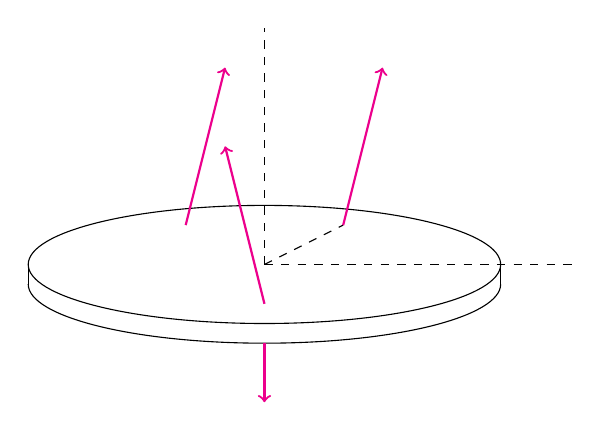
\begin{tikzpicture}
	\draw (0,0) ellipse (3 and 0.75);
	\draw (-3,-0.25) arc (180:360:3 and 0.75);
	\draw (-3,0) -- (-3,-0.25);
	\draw (3,0) -- (3,-0.25);
	\draw [dashed] (0,0) -- (0,3);
	\draw [dashed] (0,0) -- (4,0);
	\draw [dashed] (0,0) -- (1,0.5);
	\draw [->, thick, color=magenta] (1,0.5) -- (1.5,2.5);
	\draw [->, thick, color=magenta] (-1,0.5) -- (-0.5,2.5);
	\draw [->, thick, color=magenta] (0,-0.5) -- (-0.5, 1.5);
	\draw [->, thick, color=magenta] (0,-1) -- (0, -1.75);
	\end{tikzpicture}
	\caption{A Trifilar is a simple apparatus used to determine the moment of inertia for different objects.}
\end{figure}

\newpage

\subsection{Scope}



\section{Results}
Experimental characteristics of the Trifilar were measured prior to undertaking the experiment. Measurements included disk weight $m_d$; disk radius $r_d$; filament length $L$; the radius from centre of disk to middle set of holes $R$; and the radius from the disk centre to the filament base $r$. These measurements are presented in Table 1 below. To better understand where the masses were mounted on the disk, the Trifilar disk geometries are shown in Figure 3.

\begin{figure}[h]
	\centering
	\begin{minipage}{0.45\textwidth}
		\centering
		\captionof{table}{Trifilar parameter measurements}
		\begin{tabular}{lrc}
			\toprule
			Description & Value & Units \\
			\midrule
			Disk Mass $(m_d)$ & 0.200 & $\si{\kilogram}$\\
			Disk Radius $(r_d)$ & 0.140 & $\si{\meter}$ \\
			Filament Length $(L)$ & 0.450 & $\si{\meter}$ \\
			Distance to Middle Holes $(R)$ & 0.090 & $\si{\meter}$\\
			Distance to Filament $(r)$ &  & $\si{\meter}$ \\
			\bottomrule
		\end{tabular}
	\end{minipage}
	\hspace{1cm}
	\begin{minipage}{0.45\textwidth}
		\centering
		\captionof{table}{text}
		\begin{tabular}{lrc}
			\toprule
			Description & Value & Units \\
			\midrule
			Object Mass $(m_{obj})$ & 0.020 & $\si{\kilogram}$ \\
			Upper Cylinder Radius $(r_1)$ & 0.090 & $\si{\meter}$ \\
			Upper Cylinder Height $(h_1)$ & 0.007 & $\si{\meter}$ \\
			Lower Cylinder Radius $(r_2)$ & 0.090 & $\si{\meter}$ \\
			Lower Cylinder Height $(h_2)$ & 0.007 & $\si{\meter}$ \\
			\bottomrule
		\end{tabular}
	\end{minipage}
\end{figure}

\begin{figure}[h]
	\centering
	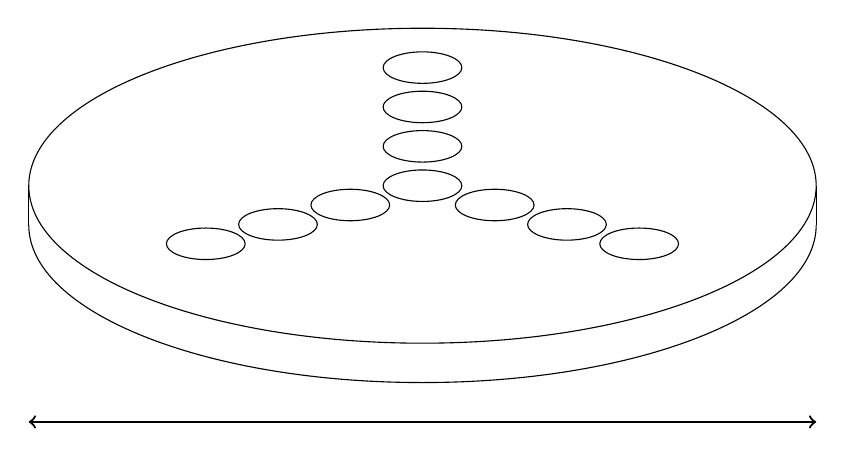
\begin{tikzpicture}
	\draw (0,0) ellipse (5 and 2);
	\draw (-5,-0.5) arc (180:360:5 and 2);
	\draw (-5,0) -- (-5,-0.5);
	\draw (5,0) -- (5,-0.5);
	
	\draw (0,0) ellipse (0.5 and 0.2);
	
	\draw (0,0.5) ellipse (0.5 and 0.2);
	\draw (0,1) ellipse (0.5 and 0.2);
	\draw (0,1.5) ellipse (0.5 and 0.2);
	
	\draw (-0.917,-0.245) ellipse (0.5 and 0.2);
	\draw (-1.835,-0.4917) ellipse (0.5 and 0.2);
	\draw (-2.752,-0.7376) ellipse (0.5 and 0.2);
	
	\draw (0.917,-0.245) ellipse (0.5 and 0.2);
	\draw (1.835,-0.4917) ellipse (0.5 and 0.2);
	\draw (2.752,-0.7376) ellipse (0.5 and 0.2);
	
	\draw[<->, thick] (-5,-3) -- (5,-3);
	\end{tikzpicture}
	\caption{Geometries of the Trifilar disk and holes where small masses were mounted.}
\end{figure}

Measurement information was also taken about the small objects, which included their mass $m_{obj}$; radius of upper cylinder $r_1$; height of the upper cylinder $h_1$; radius of the lower cylinder $r_2$; and the height of the lower cylinder $h_2$. These measurements are presented in Table 2 above. The object geometries can be seen in Figure 4.



\begin{figure}[h]
	\centering
	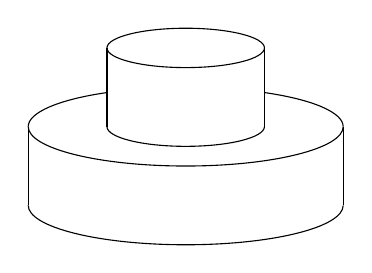
\begin{tikzpicture}
		\draw (0,0) ellipse (1 and 0.25);
		\draw (-1,-1) arc (180:360:1 and 0.25);
		\draw (-2,-1) arc (180:360:2 and 0.5);
		\draw (-2,-1) arc (180:240:2 and -0.5);
		\draw (2,-1) arc (360:300:2 and -0.5);
		\draw (-2,-2) arc (180:360:2 and 0.5);
		
		\draw (-1,0) -- (-1,-1);
		\draw (1,0) -- (1,-1);
		\draw (-2,-1) -- (-2,-2);
		\draw (2,-1) -- (2,-2);
	\end{tikzpicture}
	\caption{The small objects are essentially a small cylinder stacked on top of a larger cylinder}
\end{figure}

\begin{figure}[h]
	\centering
	\captionof{table}{text}
	\begin{tabular}{lrrrrr}
		\toprule
		Object & $(T_{10})_1$ & $(T_{10})_2$ & $(T_{10})_3$ & $(T_{10})_4$ & $(T_{10})_5$ \\
		\midrule
		Disk & 31.91 & 31.50 & 30.97 & 30.82 & 30.78\\
		Disk + 3 Objects (middle holes) & & & & & \\
		\bottomrule
	\end{tabular}
\end{figure}


\newpage

\section{Calculations}


\begin{figure}[h]
	\centering
	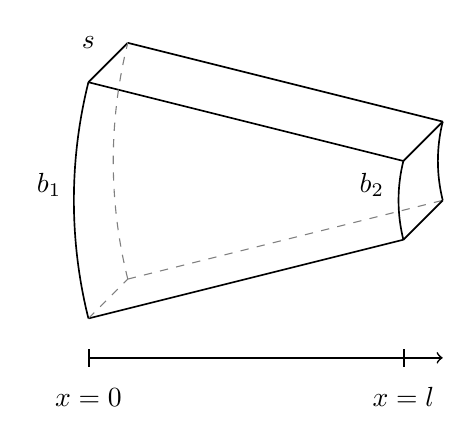
\begin{tikzpicture}
	% general shift to north east
	\coordinate (O) at (0.5,0.5);
	\draw[semithick] (0,0) -- (4,1);% bottom line in front
	\draw[dashed,color=gray] (O) -- ($(4,1)+(O)$);% bottom line in the back
	\draw[semithick] (0,3) -- (4,2);% top line in front
	\draw[semithick] ($(0,3)+(O)$) -- ($(4,2)+(O)$);% top line in the back
	\draw[semithick] (0,3) -- ($(0,3)+(O)$);% line to the back, top left
	\draw[semithick] (4,2) -- ($(4,2)+(O)$);% line to the back, top right
	\draw[semithick] (4,1) -- ($(4,1)+(O)$);% line to the back, bottom right
	\draw[dashed,color=gray] (0,0) -- (O);% line to the back, bottom left
	% the first angle is 180°+atan(0.25)
	% the second angle is 180°-atan(0.25)
	% the radius is sqrt(6^2+1.5^2)
	\draw[semithick] (0,0) arc (194.036:165.964:6.185);% left arc in front
	\draw[dashed,color=gray] (O) arc (194.036:165.964:6.185);% left arc in the back
	% the first angle is 180°+atan(0.25)
	% the second angle is 180°-atan(0.25)
	% the radius is 1/3*sqrt(6^2+1.5^2)
	\draw[semithick] (4,1) arc (194.036:165.964:2.062);% right arc in front
	\draw[semithick] ($(4,1)+(O)$) arc (194.036:165.964:2.062);% right arc in the back
	\draw (-0.5,1.7) node {$b_1$};
	\draw (3.6,1.7) node {$b_2$};
	\draw (0,3.5) node {$s$};
	\draw[|-,semithick] (0,-0.5) -- (4,-0.5);
	\draw[|->,semithick] (4,-0.5) -- (4.5,-0.5);
	\draw (0,-1) node {$x=0$};
	\draw (4,-1) node {$x=l$};
	\end{tikzpicture}
\end{figure}

\newpage

\section{Discussion}

\section{Conclusion}


\bibliography{my_bib}
\bibliographystyle{ieeetr}

\end{document}